\documentclass{article}

\usepackage{eso-pic,graphicx}
\usepackage[top=2cm, bottom=2cm, paperwidth=8in, paperheight=8in]{geometry}

\tracinglostchars=2
\usepackage{avant}
\renewcommand*\familydefault{\sfdefault}
\usepackage[T1]{fontenc}
\renewcommand{\baselinestretch}{1.2}

\renewcommand{\abstractname}{Welcome to the world of Cosmoose!}
\usepackage{xcolor}

\usepackage[parfill]{parskip}


\usepackage{verse}
\pagenumbering{gobble}
\setlength\parindent{0pt}

\usepackage{hyperref} %hyperlinks

\usepackage{graphicx}

\definecolor{darkcyan}{rgb}{0.07, 0.26, 0.26}
\definecolor{darksienna}{rgb}{0.24, 0.08, 0.08}

\newcommand{\bo}[1] {\textbf{#1}}
\newcommand{\bblu}[1] {\textbf{\textcolor{darkcyan}{#1}}}
\newcommand{\bbro}[1] {\textbf{\textcolor{darksienna}{#1}}}

\newcommand{\bckg}[1]{\AddToShipoutPictureBG*{\includegraphics[width=\paperwidth,height=\paperheight]{#1}}}

\urlstyle{same}

\begin{document}

%% title page
\bckg{img/bg}
\begin{center}
    
\includegraphics[height=.2\paperheight]{img/cclogo}

    
\includegraphics[height=.5\paperheight]{img/loading}

    \vspace{.5cm}
    {\Huge \bo{CC's Road to Stardom Guide}}
\end{center}

\clearpage

\poemtitle{Story}
\bckg{img/bg}

CC lives with the Cosmoose gang since they rescued him.
They are space pirates, on the run from the Earth's government. Is all that really important?
Not that much, since it's his Birthday! Will his dreams come true?

\begin{center}
    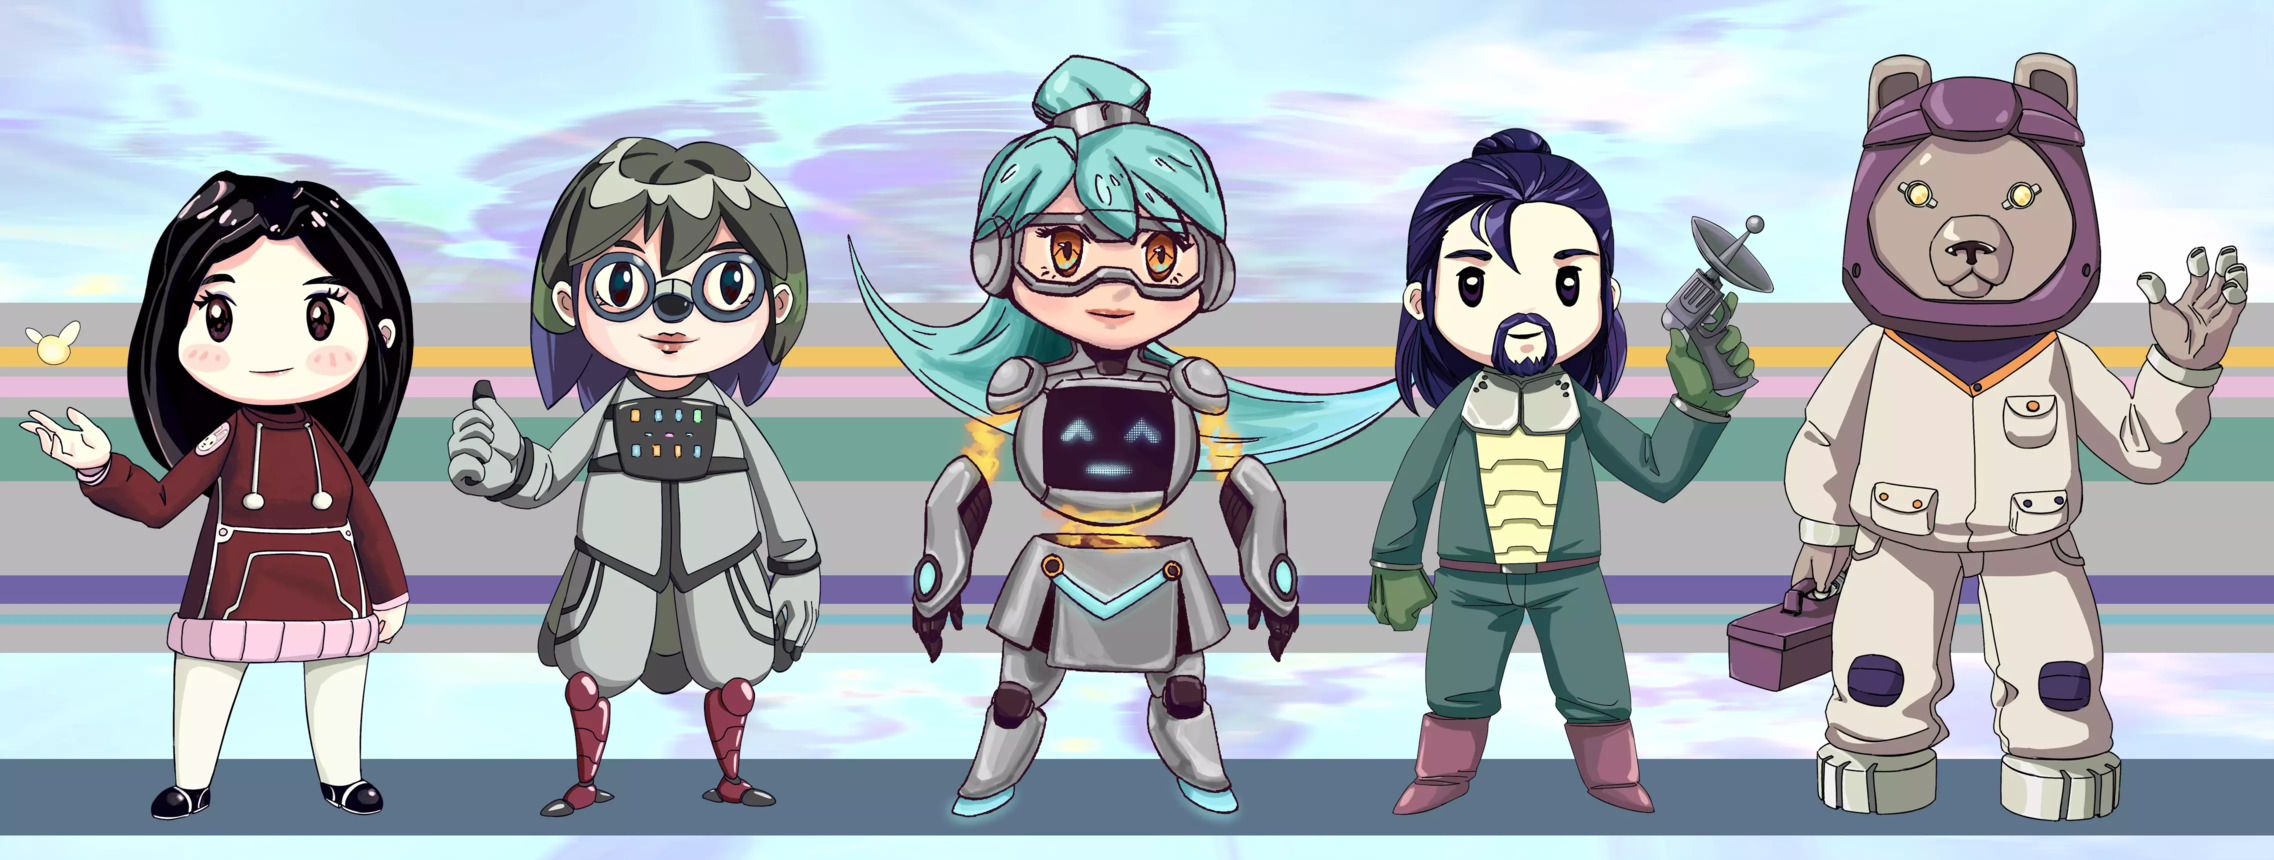
\includegraphics[height=.2\paperheight]{img/crew}
\end{center}

In this adventure, you play as CC.
Here are all of your friends, from left to right:
\begin{itemize}
    \item Florrie, the nicest person on the ship! But she left for a programming exam...
    \item June, the inventor, who just gave you a mirror! What a good idea, we all need more beauty in our life!
    \item 7Cs, the ship's AI, who knows a lot about everything, because she's a robot.
    \item Ru D., the captain, who is most likely always found in the gaming room.
    \item Wool, who's probably nice, you're not sure, because you don't really get what he says.
\end{itemize}

With their help, you will become the number 1 idol in the universe. Or so is the plan.

\clearpage
\poemtitle{Playing the game}
\bckg{img/bg}

This is a classical text adventure game.
To play, you need to input a \texttt{VERB} and a \texttt{SUBJECT}, or simply a \texttt{VERB}.

You'll need to \texttt{EXAMINE} your surroundings and the various objects you can find,
for example \texttt{EXAMINE LAPTOP}.
Various synonyms are accepted, as well as some shortcuts, like \texttt{X} for \texttt{EXAMINE}.
The words \texttt{LAPTOP} and \texttt{COMPUTER} are synonyms, as are \texttt{COW} and \texttt{BOUNCYBULL}.
So \texttt{X COMPUTER} would have done the same thing.
It's very logical!
The programmers might have too limited a vocabulary, so they probably did NOT got ALL synonyms.
There are many words. If your favorite didn't make it, try a different one.

If you forgot the location description, simply \texttt{LOOK} around you to see it again.

You can \texttt{GIVE} or \texttt{GET} objects. To check the objects you have on paw,
use \texttt{INVENTORY} (or \texttt{I}).

To move on the map, you can use the cardinal directions, \texttt{NORTH}, \texttt{EAST},
\texttt{SOUTH} and \texttt{WEST} (or shortcuts \texttt{N}, \texttt{E}, \texttt{S}, \texttt{W});
there are some places you can \texttt{ENTER} or \texttt{EXIT}.
Just don't get lost! If you found a map, you can \texttt{USE MAP} to know where you are.
Handy! (pawy!)

Type \texttt{HELP} to get some \texttt{HELP}.
If you need help with a puzzle, type \texttt{HINT} and hope that the programmers put some helpful message.
If this is still too obtuse, you can just check the guide below to check the solution.

\clearpage

\clearpage
\poemtitle{Game Guide 1/2}
\bckg{img/bg}

\bblu{\bo{Beware, the solutions to puzzles are ahead! Only use this if you're blocked.}}

You start in your room, where the mirror that June gave you is making you feel quite uncomfortable.
Pigeons would be more popular than you? Impossible.
You need the crew to help you find the truth, and help you become famous.

You go \texttt{SOUTH} to the common room.
There's nobody, but your best friend Florrie left her laptop.
Inadvertently, you \texttt{EXAMINE} her laptop and see she left a password hint.
There has to be useful info on it. The hint talks about grey birds.
Knowing her, it can only be the \texttt{PIGEON} we are talking about.
But the information you get is scary... she's OBSESSED with pigeons!

Let's ask Wool, who's always level-headed. He's just \texttt{WEST} of the common room.
After a \texttt{TALK}, he does not seem interested in pigeons, but in logic.
He won't let you go before answering his logic puzzle... luckily there are only two possible answers.
If you \texttt{GUESS RED}, you're free to go!

Wool said solving puzzles is popular.
Let's test that hypothesis with Ru D., just \texttt{SOUTH} of here.
The hall seems a bit gloomy despite the "Party Planet" neon lights.
You can hear music from the inside, so you \texttt{ENTER}.
Ru D. is gaming, as usual. When you \texttt{TALK} to him, he tells you he has a predicament!
He doesn't know which mini-game to choose to earn enough points to win a bet in his game.
That's just a puzzle for someone like you!
After a short mental computation, you \texttt{GUESS 3}. That's it, problem solved!
But now, Ru D has gone back entirely focused on his game and is not interested in you anymore.
That must mean it's not sufficient to become famous...

You decide do ask someone more reliable.
Since 7Cs is a robot, she knows much more about everything.
After an \texttt{EXIT} from the gaming room, you just need to go \texttt{EAST}.
She is in the Crispy Yard, chilling close to the chicken tree.
When you \texttt{TALK} to her, she ask you to find by yourself which channel is the most popular one.
You ask for a \texttt{CLUE B}, \texttt{CLUE C}, then correctly \texttt{GUESS C}!
She then explains complicated stuff to help people.
Definitely not going to help you become famous.

\clearpage
\poemtitle{Game Guide 2/2}
\bckg{img/bg}

You leave \texttt{NORTH} for the common room,
and find June hanging around with E the pigeon, who has a super-popular channel!
You \texttt{TALK E}, who basically tells you having channel is like some sort of job.
Well. When you \texttt{TALK JUNE}, she admits to bugging Florrie's laptop with her pigeon software.
The mirror programming was also her doing.
All this ado about pigeons was just June's twisted view of reality!

Up to now, the day has been only disappointments.
You don't have a clue how to become famous, your best friend is away, and you had no cake.
You're tough, but start to cry nonetheless.
Then E starts mocking you, saying that he got that on video! The horror!
While you get in your safety blanket, June gives you a magic beak that makes you a hero.
You \texttt{THANK JUNE}, when E who was still laughing starts choking on his popcorn!

To help him, you have to remember the first aid maneuver 7Cs explained to you just before.
You have to give 5 back blows, 5 abdominal thrusts, and loop until the popcorn is dislodged.
A true hero!

You don't even have time to celebrate as alarms go off!
Something is wrong, the ship is going through an asteroid belt with strong space winds,
that is swarming with enemy drones! A hero has to guide the ship through this ordeal.
You \texttt{ENTER} the command booth, and start looking where to go.
Your logical skills, boosted by the beak power, makes you see the path in a flash!

\texttt{E S S E S W W S E E E N N N E S S S} \\
Phhhew! You did it!

Florrie just came back, and you tell her all that happened.
She's happy to hear that so she gives you the only question she struggled with during her exam.
You decypher the message, \texttt{OPENSOURCENOW} and now you've even helped her!
With that, you can \texttt{EAT CAKE} and celebrate with all your friends!

\clearpage

\poemtitle{Credits \& Special Thanks}
\bckg{img/bg}

This game is made in Adventuron, a tool you can make to do your own games!
Go visit \href{https://adventuron.io/documentation/tutorial-a.html}{Adventuron Tutorial}!

This adventure would have not come to life without the existence of \href{https://indiemusicfeedback.com}{Indie Music Feedback}.
So we want to thank all \bbro{IMFers} for the encouragement they offered, and for the fun they are bringing to our lives.

We also want to thank our playtesters, who gave very useful remarks.
We are particularly grateful to \href{https://daphnecerez.carrd.co/}{Daphne},
Gaby, Jorchime, JJYY and Mélanie for their precious advice.

Made with love by \href{https://cosmoose.org/}{Cosmoose} \& \href{https://okfeather.com/}{OK Feather}.\\
Original Music: \href{https://linktr.ee/dhxp}{DHXP}.\\
Illustrations: \href{https://twitter.com/wooliondraws}{Woolion}.\\
Programming, Booklet: Dova Lin, E, Woolion.

You can find the source of the game and this booklet on
\href{https://github.com/cosmoosic/cc-star}{Cosmoose's Github}.

\vspace*{\fill}

\begin{center}
    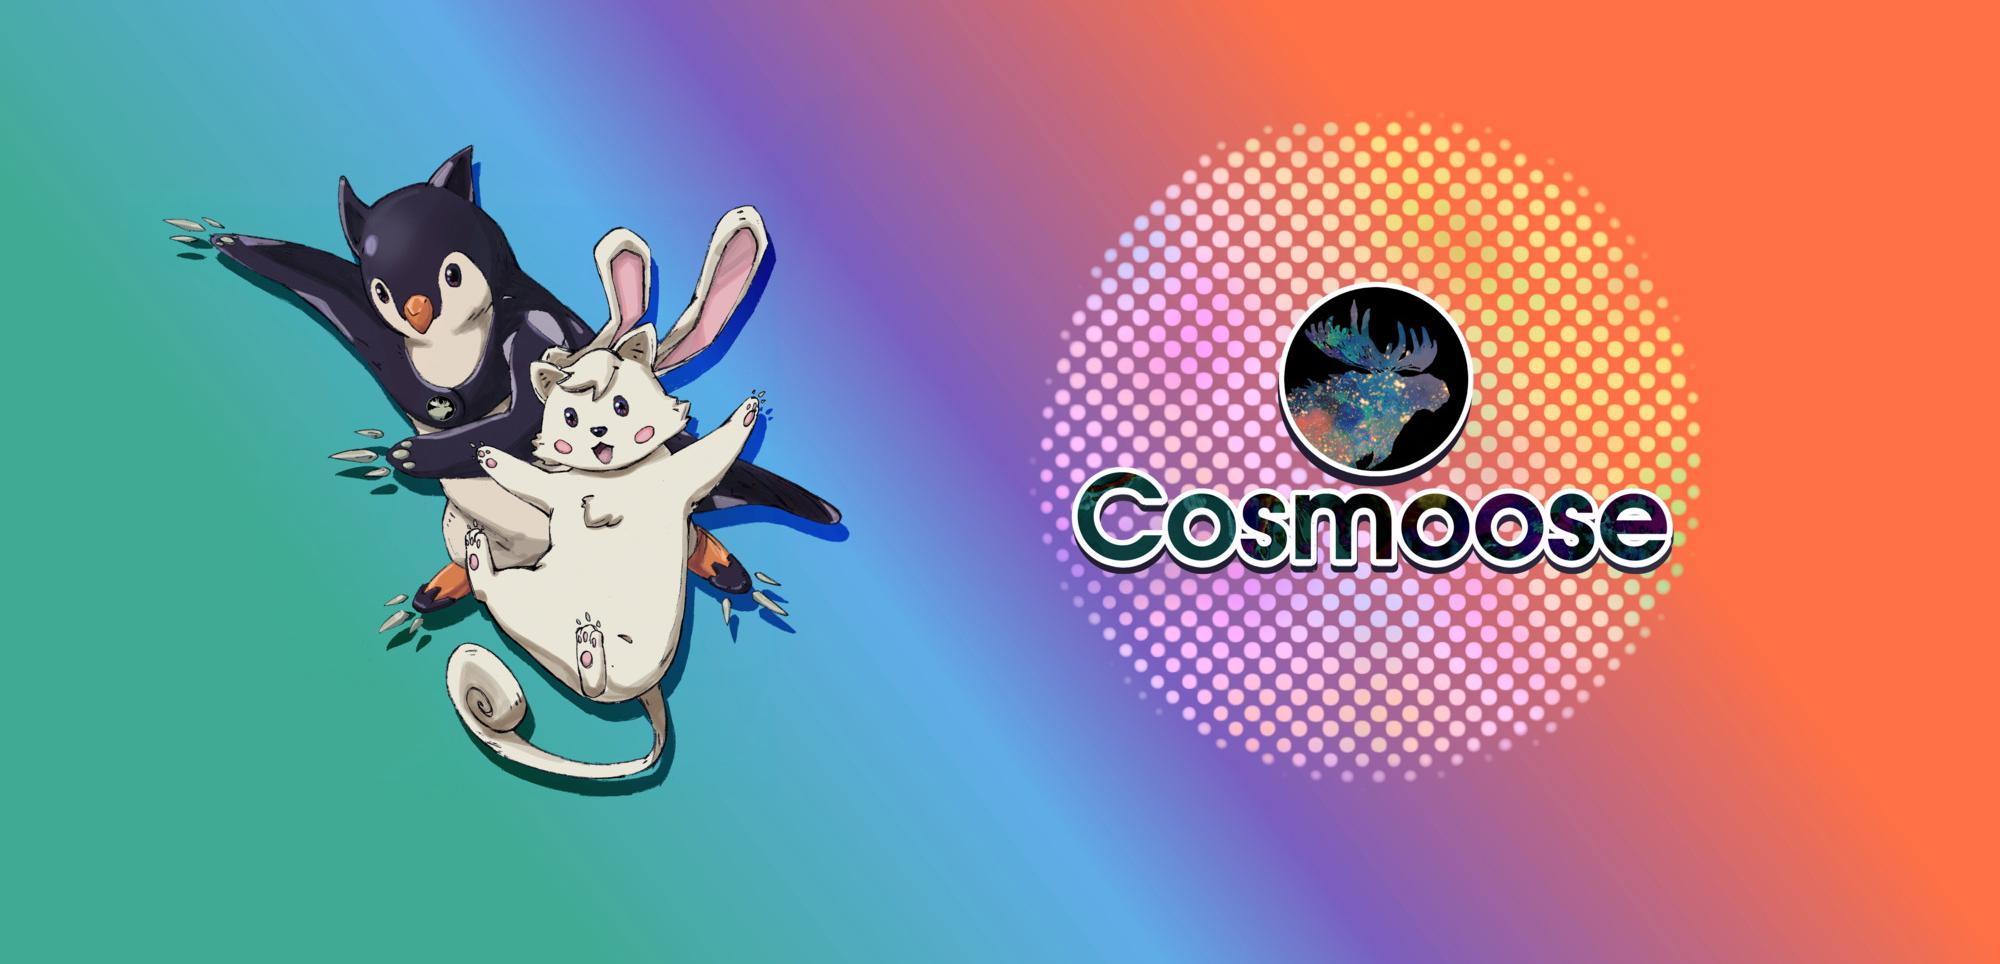
\includegraphics[height=.35\paperheight]{img/ccend}
\end{center}


\clearpage


\end{document}

